\documentclass[letterpaper,11pt]{article}
\usepackage[T1]{fontenc}
\usepackage[utf8]{inputenc}
% see https://qiita.com/zr_tex8r/items/cdaac1500718eb9fa330
% \usepackage{CJKutf8}
\usepackage[whole]{bxcjkjatype}
\usepackage{hyperref}
\usepackage{tabularx}
\usepackage{helvet}
\usepackage{times}
\usepackage{courier}
\usepackage{relsize}
\usepackage{graphicx}
\usepackage{xspace}
\usepackage{mycv}
\usepackage[top=15mm,left=15mm,right=15mm,bottom=15mm]{geometry}
\usepackage[subsectionbib]{bibunits}
\usepackage{chicago}            %required for chicago bib style
\defaultbibliographystyle{plainyr-rev}
\defaultbibliography{asai-references}
\bibliographyunit[\section]

\usepackage{xparse}
\RenewDocumentCommand{\subsection}{s m}{}

\begin{document}

\pagestyle{empty}

%Ueberschrift
\begin{center}
{\huge\textsc{Curriculum Vitae}}
\vspace{0.7\baselineskip}

{\Large\textsc{Masataro Asai, Ph.D}}
\vspace{0.5\baselineskip}

\small

 Affiliations: MIT-IBM Watson AI Lab, IBM Research Cambridge.
 Sex: Male. Date of Birth: March 28th, 1990. Nationality: Japanese.
 Address: 22 Water St APT 813 Cambridge, MA 02141, U.S.A.
 Phone: +1-857-999-5722.
 Email: guicho2.71828@gmail.com
\end{center}

\section{Main Research Interest}

\textbf{Neural-Symbolic Systems (Machine Learning + Classical AI) for domain-independent search/planning/reasoning.}
With the main background in Classical Planning and Heuristic Graph Search,
 my recent interests involve two key subareas:
(1) \red{Automatic identification of discrete symbolic representation for planning}, i.e.,
symbol grounding and knowledge acquisition, with the help of Deep Neural Networks and Bayesian generative modeling.
(2) \blue{Use of machine learning and statistical modeling for learning a heuristic guidance} for problem solving and enhancing search efficiency.

\begin{figure*}[h]
 \centering
 \begin{minipage}{0.4\linewidth}
 \includegraphics[width=\linewidth]{img/mnist-plan.pdf}
 \end{minipage}
 \hspace{0.1\linewidth}
 \begin{minipage}{0.4\linewidth}
 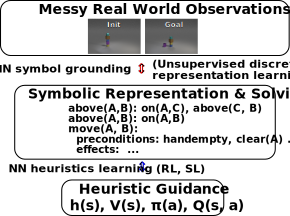
\includegraphics[width=\linewidth]{img/plan.pdf}
 \end{minipage}
 \caption{
 \textbf{(Left)} Result of visually solving 8-puzzle using a learned discrete representation and a classical planner.\\
 \textbf{(Right)} Cognitive architecture can have neural components for two distinct purposes: \red{Perception} and \blue{heuristics}.
 }
\end{figure*}


\section{Education}

\begin{CV}
 \item[04/2015--03/2018] \textit{Ph.D}.
 Artificial Intelligence, Heuristic Search, Planning, Scheduling, Optimization.
 Thesis title: \emph{Diversification Mechanisms for Best-First Search};
 Advisor: A. Fukunaga

 \item[04/2013--03/2015] \textit{M.A}.
 Artificial Intelligence, Heuristic Search, Planning, Scheduling, Optimization.
 Thesis title: \emph{Automated Cyclic Planning for Large Scale Planning Problems};
 Advisor: A. Fukunaga

 \item[04/2009--03/2013] B.Eng in Traffic Simulation.
 Multi-Agent Model, Spatial Search.
 Thesis title: \emph{Distributed Cooperative Agents in Microscopic Traffic Simulation using St-RRT};
 Advisor: S. Yoshimura. H. Fujii.
\end{CV}


\section{Work Experience}

\begin{CV}
\item[07/2019--present.] Staff Research Scientist (PI) at \textbf{MIT-IBM Watson AI Lab, IBM Research Cambridge} (Full Time).

\item[04/2018--07/2019.] Research Staff Member (PI), Embodied Learning Group, \textbf{IBM Research Tokyo} (Full Time).

\item[08/2016--11/2016] Research Intern, \textbf{IBM Research Ireland.}
 Project name: Robust Activity Planning and Scheduling with Multi-Modal Travel.
 Developed an efficient algorithm for multi-worker routing.

\item[04/01/2016--03/31/2018] Research Fellow (DC2), Japan Society for the Promotion of Science.

% \item[03/2014--09/2014] Internship at LogicVein.inc,
%  % LogicVein is
%  a developer of a Configuration Management System
%  for network devices.
%  % , an award-winning software that allows the users to
%  % efficently manage the complex network configurations of remote routers and switches.
%  % Useful batch orders can be triggered by their intuitive graphical interface.
%  Worked on % . The materials
%  % consist of: advertisement leaflets, blog articles and
%  a technical product manual (>200 pages long) %  The materials
%  % contain both the Japanese and English documents. Some staff are
%  % native English speakers born in United States, who checked and highly
%  % evaluated the quality of the English translation.
%  % and converted it into
%  % i also converted the Microsoft Word documents into
%  % plain-text documents to set up a publishing system.  It compiles the
%  % document into a \LaTeX{}-based pdf and multiple
%  and its HTML5 conversion.

% \item[04/2013--08/2013] Teaching Assistant in ``Experiments in
%  Information and Environmental Sciences'', under
%  Assoc.\ Prof.\ Haruo Saito.
%  % Students are required to
%  % conduct a specific experiment each week. Experiments include reading
%  % the data from the various sensors and importing it to a computer,
%  % during which the students are required to make use of digital circuits.
%  % Tasks also include measuring the output of comparators, invert
%  % amplifiers and filters that must be built by the students.
%  Students have assembled and calibrated the analog or digital
%  circuits to read the physical values of experimental equipments.

% \item[04/2012--08/2012] Teaching Assistant in ``Field Work -
%  Introductory Course on Automobiles'', under
%  Prof.\ Kohei Kusaka.
%  % The students learn the mechanism and the engineering
%  % design decision of vehicles through vehicle maintenance experience.
%  % prepared the maintainance materials such as lubricant, sealing and
%  % oil filters, moved the vehicle which will be used for maintainance, and
%  Lectured on basic safety measure and the mechanism of vehicles.

% \item[12/2011--09/2012] Internship at Metamoji.inc.  Prototyped a
%   drawing-chat system for iPad. Both the server/client sides are
%   written in Javascript with Node.js and Titanium Mobile.
\end{CV}

\section{Journal Publications, Book Chapters}

\nocite{Asai2022}
\nocite{Asai2021}
\nocite{Asai2017}
\putbib

\section{Conference Publications ($^*$: Presenter)}

\nocite{wissow2023scale}
\nocite{carlos2024admissible}
\nocite{Asai2022b}
\nocite{Asai2022c}
\nocite{Asai2020}
\nocite{Asai2019a}
\nocite{Asai2019b}
\nocite{Asai2018}
\nocite{Asai2017e}
\nocite{Asai2017b}
\nocite{Asai2016b}
\nocite{Asai2016}
\nocite{Asai2015}
\nocite{Asai2014}
\putbib

\section{Workshop and Other Publications ($^*$: Presenter)}

\nocite{wissow2024extreme}
\nocite{asaiphd}
\nocite{Asai2022d}
\nocite{asai2021generating}
\nocite{Asai2020b}
\nocite{Asai2020c}
\nocite{Asai2019c}
\nocite{Asai2018b}
\nocite{Asai2016c}
\nocite{Endo2016}
\nocite{Asai2014b}
\putbib


\section{Patents}

\begin{CV}
 \item Discrete feature representation with class priority, US Patent App. 16/290250
 \item Permutation-invariant optimization metrics for neural networks, US Patent App. 16/366678
 \item Discovering higher-level actions from expert's action demonstration, US Patent App. 16/419183
 \item Symbolic model training with active learning, US Patent App. 17/132776
\end{CV}

\section{Grants}

\begin{CV}
 \item[09/2022-09/2024] DTIC contract FA8075-18-D-0008, Task Order FA807520F0060, Task 4 - Autonomous Defensive Cyber Operations (DCO) Research \& Development (R\&D).
\end{CV}

\section{Awards}

\begin{CV}
 \item[06/2022] ICAPS 2022 Outstanding PC and SPC Award (Outstanding Program Committee Members).

 \item[04/2016--] Research Fellow (DC2), Japan Society for the Promotion of Science.
 (Equivalent of NSF Grant in Japan; stipends and individual research budget of 10000 USD/year.)
 \item[03/2017]
 JSAI Annual Conference Student Award, The Japanese Society for Artificial Intelligence.
\end{CV}

% \section{Technical Skill}
%
% \begin{CV}
%  \item[Programming Paradigm:] %Familiarity with all of:
%  Object-Oriented programming,
%  Functional programming,
%  Logic / Rule-based programming,
%  Metaprogramming, low-level optimization,
%  Domain Specific Language(DSL) development, compile-time optimization.
%  \item[Development:] Git, GitHub Flow, Test-Driven Development and Continuous Integration (Travis-CI / CircleCI).
%  \item[Languages:]
%  (Professional) Common Lisp, C++, Bash, Python, Javascript / Coffeescript, C,
%  (Intermediate) Java,
%  (Elementary)   Ruby
%  % \item[Hardware skill:]
%  % Digital and Analog circuits, microcontrollers(Arduino,PIC), machining, welding
%  \item[Frameworks:] Pytorch, TensorFlow/Keras, Cloud (Amazon AWS, Torque/PBS, OpenLava, cfncluster),
%  Node.js% , Titanium Mobile
% \end{CV}

\section{Language}

\begin{CV}
 % \item[Japanese:] native
 \item[English:] TOEFL 105/120 (Reading:29/30, Listening:29/30,
 Speaking:22/30, Writing:25/30, Dec 2014).
 % I enjoy daily discussion on Reddit, Github, Skype and IRC channels.
\end{CV}

\section{Invited Talks / Community Services / Other activities}

% (2021/09/27) Invited talk at University of New Hampshire
(2024/09/05-06) Invited talk at SIG-FPAI (Special Interest Group on Fundamental Problems in Artificial Intelligence),
Iwakuni, Japan. \url{https://sig-fpai.org/past/fpai129_cfp.html}

(2021/07/15) Invited talk at RSS 2021 Workshop on Declarative and Neurosymbolic Representations in Robot Learning and Control,
in 2021 Robotics: Science and Systems (RSS) Conference. \url{https://dnr-rob.github.io/}

(2019/12/10) Featured in Nikkei Business Publications \url{https://xtech.nikkei.com/atcl/nxt/mag/rob/18/012600001/00044/}

(2016-) PC / SPC member roles in AI conferences (AAAI, IJCAI, ICAPS, AAMAS, Neurips, ICLR)

(2019) \href{https://github.com/numcl/numcl}{numcl},
A Numpy clone in Common Lisp. Was temporarily \#5 on Hacker News and gained 300+ stars.

(2015) \href{https://github.com/guicho271828/eazy-opencl}{eazy-opencl}
: Common Lisp interface to OpenCL 2.0 (GPGPU language similar to CUDA).

(2015) Contributer of \href{https://github.com/pocl/pocl}{POCL},
a vender-agnostic Portable OpenCL implementation in C and C++.

(2015) \href{https://github.com/guicho271828/trivia}{trivia},
\href{https://github.com/guicho271828/trivia.balland2006}{trivia.balland2006}
: An extensible and fast pattern matching compiler in Common Lisp.

% (2012) Macascript : a homoiconic language that compiles into javascript.

(2013--2018)
 Compute cluster maintainance and management (80 cores) with NFS/NIS/Torque-PBS.
 Live monitoring/power consumption management.
 Secure VPN network over the campus.

(2011--2012) Mechanical engineering under project professor Kohei Kusaka (former World Rally
 Championship co-driver):
 Full engine modification \& rebuilding of 1.8 liter Mazda BP engine,
 fuel map / ignition timing optimization, map visualization and
 variable resonance intake system (Arduino).

(2011) Certification in ``basic course on machining technique'' by Prof. Ryu Chikayama.

% (2005--2007) Development of Bipedal robot with embedded microcontroller
% (Microchip\textregistered PIC and analog servo motors)

% One of my planning domain CELL-ASSEMBLY is added to SIGAPS ``Real and
% Realistic Planning Domains'' by Patrik Haslum at
% \url{http://users.cecs.anu.edu.au/~patrik/sigaps/index.php?n=Main.RealDomains}


% \section{Undergraduate Thesis Abstract}
%
% {\small
% In large-scale traffic simulation,
% microscopic multiagent model simulates the behavior of each car (an agent)
% to produce the macroscopic emergent phenomena, e.g.\  traffic-jams,
% % The accuracy of the model are validated through
% % the comparison between the k-q (traffic density to average velocity)
% % curves of simulated and actual environments.
% % which can be heavily affected by the agent behavior.
% and the development of realistic agent model is the key to maintain the simulation accuracy.
% We proposed a coorperative agent model based on Spatiotemporal RRT(St-RRT)
% and evaluated the effectiveness of our approach.
% }
%
% \section{Masters Thesis Abstract}
%
% {\small
% In Automated Planning \& Scheduling (P\&S),
% domains such as factory assembly requires the program to
% assemble many identical instances of a particular product.
% While modern classical
% planners can generate assembly plans for single instances of a complex
% product, generating plans to manufacture many instances of a product is
% beyond the capabilities of standard planners. We proposed ACP, a system
% which, given a model of a single instance of a product, automatically
% reformulates and solves the problem as a cyclic planning problem.  We
% showed that our ACP system can successfully generate
% cyclic plans for problems which are too large to be solved directly
% using standard planners.
% }

% \begin{figure}[h]
%  \centering
%  \includegraphics[width=0.7\linewidth]{img/mandrill-intro.pdf}\\
%  \includegraphics[width=\linewidth]{img/mandrill-plan.pdf}
%  % \includegraphics[width=0.9\linewidth]{img/static/lenna.png}
%  \caption{Another 8-puzzle result from \cite{Asai2018}}
% \end{figure}
%
% \begin{figure}[h]
%  \centering
%  \includegraphics[width=\linewidth]{img/hanoi3.pdf}
%  \includegraphics[width=\linewidth]{img/hanoi4.pdf}
%  \caption{The same system can solve Tower-of-Hanoi without human supervision / assigned labels nor any architectural change..}
% \end{figure}
%
% \begin{figure}[h]
%  \centering
%  \includegraphics[width=\linewidth]{img/lightsout_new4x4.pdf}
%  \includegraphics[width=\linewidth]{img/lightsout_twisted_new4x4.pdf}
%  \caption{The same system can solve 4x4 LightsOut (\url{https://en.wikipedia.org/wiki/Lights_Out_(game)}) as well as its ``twisted'' version (Bottom).
% The goal state has only a small noise, but it was normalized and enhanced by the plotting library.}
% \end{figure}

\end{document}
